
\documentclass[twoside]{article}


% ------
% Fonts and typesetting settings
\usepackage[sc]{mathpazo}
\usepackage[T1]{fontenc}
\linespread{1.05} % Palatino needs more space between lines
\usepackage{microtype}
\usepackage{textcomp}


% ------
% Page layout
\usepackage[hmarginratio=1:1,top=32mm,columnsep=20pt]{geometry}
\usepackage[font=it]{caption}
\usepackage{paralist}
\usepackage{multicol, hyperref, graphicx}
\usepackage{parskip}

% ------
% Lettrines
\usepackage{lettrine}
\usepackage{color}

% ------
% Abstract
\usepackage{abstract}
	\renewcommand{\abstractnamefont}{\normalfont\bfseries}
	\renewcommand{\abstracttextfont}{\normalfont\small\itshape}


% ------
% Titling (section/subsection)
\usepackage{titlesec}
\renewcommand\thesection{\Roman{section}}
\titleformat{\section}[block]{\large\scshape\centering}{\thesection.}{1em}{}


% ------
% Header/footer
\usepackage{fancyhdr}
	\pagestyle{fancy}
	\fancyhead{}
	\fancyfoot{}
	\fancyhead[C]{ $\bullet$ Draft $\bullet$}
	\fancyfoot[RO,LE]{\thepage}

% My Shortcuts 

%useful shortcuts
\def\R{\ensuremath{\mathbb{R}}} %\ensuremath adds math mode, if forgotten
\def\Q{\ensuremath{\mathbb{Q}}}
\def\N{\ensuremath{\mathbb{N}}}
\def\Z{\ensuremath{\mathbb{Z}}}
\def\C{\ensuremath{\mathbb{C}}}

%shorcuts with arguments
\newcommand{\abs}[1]{\left\vert#1\right\vert} %nice absolute values
\newcommand{\bt}[1]{\textbf{#1}} %bold
\newcommand{\eq}[1]{\begin{align*}#1\end{align*}} %aligned equations
\newcommand{\cb}[1]{\centerline{\fbox{#1}}} %centered box
\newcommand{\bp}[1]{\fbox{\parbox{0.8\textwidth}{#1}}} %box paragraph
\newcommand{\norm}[1]{\left\lVert#1\right\rVert} %vector norm
\newcommand{\notimplies}{% does not imply
  \mathrel{{\ooalign{\hidewidth$\not\phantom{=}$\hidewidth\cr$\implies$}}}}
\renewcommand{\eq}[1]{\begin{align*}#1\end{align*}} %aligned equations

%colors
\definecolor{javagreen}{rgb}{0.25,0.5,0.35} %dark green color
\definecolor{lightblue}{rgb}{0.149,0.545,0.824} %solarized blue
\definecolor{sred}{rgb}{0.863, 0.196, 0.184} %solarized red

\newcommand{\blue}[1]{{\leavevmode\color{lightblue}{#1}}} %solarized blue 
\newcommand{\green}[1]{{\leavevmode\color{javagreen}{#1}}} %command for green
\newcommand{\red}[1]{{\leavevmode\color{sred}{#1}}} %solarized red
\newcommand{\gray}[1]{{\leavevmode\color[gray]{0.5}{#1}}} %gray text

%environment
\newcommand{\tab}{\phantom{ssss}}
%----------------

% ------
% Clickable URLs (optional)
\usepackage{hyperref}

% ------
% Maketitle metadata
\title{\vspace{-5mm}%
	\fontsize{24pt}{12pt}\selectfont
	\textbf{What's So Special About Philosophy?} 
	}	
\author{%
\fontsize{14pt}{14pt}\selectfont
	Unraveling Wikipedia's First Link Network \vspace{-2mm}\\
	}
\date{}

%figures
\usepackage{graphicx}
\usepackage{caption}
\usepackage{subcaption}
\usepackage{float}


%%%%%%%%%%%%%%%%%%%%%%%%
\begin{document}
\maketitle
\thispagestyle{fancy}
%========================ABSTRACT====================================

\begin{abstract}
\fontsize{12pt}{12pt}
\selectfont

Apples, oranges, and the most obscure Dylan song too---is everything a few clicks from Philosophy? In Wikipedia, the surprising answer is yes. 

Wikipedia is the largest, most meticulously indexed collection of human knowledge ever amassed. Yet, we have never closely examined the naturally formed web tying one entry to another. By following the first link in an article, we connect entries to form a directed network within Wikipedia: Wikipedia's First Link Network. Here we study Wikipedia's First Link Network for insight into how we link the largest collection of topics, ideas, people, objects, and events.  Structurally, we discover Wikipedia's First Link Network is by many metrics a scale-free network with Philosophy at a salient center by many orders of magnitude. 
We also learn the network generalizes specific events, objects, or phenomena to broader basins around Community, State, and Science. 


\green{
conclusions to mention
\begin{itemize}
    \item finding many small-world phenomenan in the number of first links flowing through a page, the path lenghts, and ...\\
    \item also cementing Philosophy as an extremely peculiar article, orders of magnitude away from other article in Wikipedia by our metrics.
    \item links generalize specific event, object, or phenomemon to a broader concept. Mention synonyms
\end{itemize}
}
\end{abstract}

\fontsize{11pt}{11pt}
\selectfont

%========================INTRODUCTION====================================
At no point in history has a larger or more meticulously indexed collection of human knowledge existed.
((cite))
In amassing such an awe-inspiring collection, we formed an equally impressive web. 
Through the efforts of millions of individuals, working independently,
((cite))
we naturally linked topics, inventions, people, objects, places, and events across space and time.
The web we weaved, and continue to weave, is a wealth of information not only about those notable inventions, 
places, figures, and ideas, but also about \textit{relationships} among them.
Here we study the relationships in this naturally arising web through the hyperlinks connecting one article to another.

We build Wikipedia's First Link Network by following the first link, not in parenthesis, inside the main body of each article in the English version of Wikipedia. 
For the directed network to meaningfully reflect how we associate one article to another, we exclude links in parenthesis, 
disregarding pronunciation keys or disambiguations.
We also exclude any links in the side-bar elements, as well as any links to external pages, files, or WikiMedia 
projects outside of Wikipedia (such as Wiktionary).
((footnote: this also stays true to the original blog post))
The result is a directed network placing every article in a broader web of ideas.


%===========================Data_and_Parsing================================
\section{Constructing the First Link Network}

To map Wikipedia's First Link Network, we use the freely-available XML dump of the English Wikipedia. 
Rather than rely on a sample of articles from which to generalize, we opted to process the entirety of Wikipedia, 
eliminating any statistical error due to sampling.
We analyze the snapshot provided on November 2014, representing the state of Wikipedia at the time.
The November raw dump consists of 11 million articles: 4.7 million unique articles along with redirects
and disambiguations.
Knowing Wikipedia is an ever-evolving project with 10 edits every second and 750 new articles per day on average
((cite)), our aim is to characterize the dynamics of the First Link Network, not record a particular link between one
article and another.

Wikipedia renders and stores articles in MediaWiki markup, a markup language with syntax and keywords to format and mark elements in a page. Along with special syntax for links, MediaWiki markup includes templates for audio files, images, and side-bar
information.
While a human can accurately identify the first link, to map the entire First Link Network of 11 million articles, we programmatically untangled the body text from side-bar, header box, and bad link elements.

While some libraries exist for MediaWiki Markup, we opted to develop our own algorithm for parsing the first link in the XML version of each article. 
\footnote{Approaches using existing libraries led to several bugs 
including trouble with nested links, nested parenthesis, unclosed tags, escape characters 
as well as compatibility with other libraries used to parse the XML.}
Our parsing algorithm aimed to: 
1. squash the initial bugs 
2. eliminate the need for several passes. 
To process an article with one pass, we developed a hierarchical system of flags:
\begin{itemize}
    \item[Flag 1:] inside template?
    \begin{itemize}
        \item[Flag 2:] inside <ref>, <div>?
        \begin{itemize}
            \item[Flag 3:] inside ()?
        \end{itemize}
    \end{itemize}
\end{itemize}
((better graphic to come))

The algorithm loops in three-character chunks to account for potentially nested elements, 
shifting by one character steps through the article markup.
If any markup triggers for a flag are detected a flag is raised. 
Once a flag is raised, we stop processing and proceed to the next character
until the flag's closing markup is detected.
A first link is identified only if Flags 1, 2, and 3 are all off.
In this case, the entire link is retrieved. 
We then confirm the link is valid by filtering for MediaWiki keywords indicating external page or other projects
as well as common file extensions for 
((cite))
images, audio files, and the like.
The first link of an article is then the earliest valid link with unraised flags.

To process the entirety of Wikipedia, we distributed the parsing and processing of the XML dump
across 112 cores of the UVM supercomputer cluster
((cite))
We then joined the results to form a hash table containing every Wikipedia article and its corresponding
first link. The resulting network is the basis of our analysis.


%========================Traversing the Network====================================
\section{Traversing the Network}

To understand the structure of Wikipedia's First Link Network, we
aimed to characterize the dynamics of the flow from one article to another. 
Do links tend towards a particular article, group of articles, or groups of articles? 
What is the flow of links through a typical article?
What types of cycle (loop) structures exist in the network?
What are typical paths from one article to loop or a dead end (invalid link)? 
((add other questions we end up answering))
Are there exceptionally long or short paths? 
Are there articles funneling the flow of links towards a particular path?
In answering these questions about the directed network, we aimed to characterize 
how so many independent articles relate to each other.

The n-degree, or number of links directly pointing to a particular article,
while a natural measure, fails to fully capture the dynamics needed to answer these questions.
The n-degree measures only the particular set of links to a particular article, 
rather than the richer dynamics of how the links flow through the network: 
where articles tend, what the typical and atypical 
paths through the network are, which articles funnel relatively more links and so on. 

Consequently, we developed three metrics to capture the dynamics of how the First Links flow. 
First, we traverse the network to measure the accumulated number of visits each article receives as we 
follow every possible link path: \\

\begin{figure}[H]
\centering
    \caption{traversing the network}
\begin{subfigure}[b]{0.8\textwidth}
    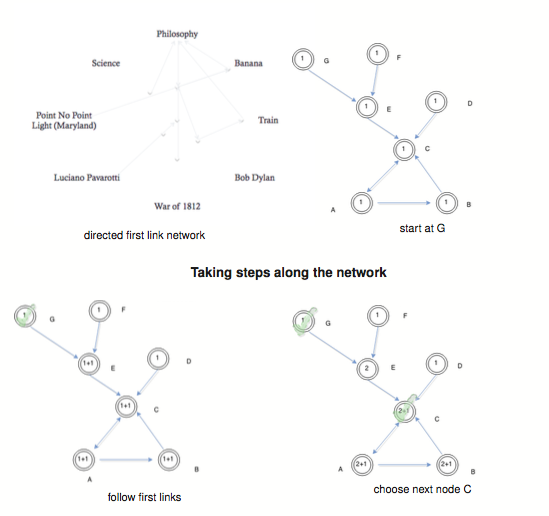
\includegraphics[width=\textwidth]{graphics/traverse_algo.png}
\end{subfigure}
\end{figure}

((diagram and explain))

Second, we traverse the network in the same manner, but end our paths once we enter a cycle (loop in the network).
We call the accumulated number of visits, the number of traversal funnels, because we quantify
which articles funnel more link paths in particular direction or cycle.

Finally, we can also track the path length, or the number of links until we repeat an article or reach an invalid link.
Additionally, by recording the history of articles we traverse to map cycles in the network.
The three metrics: traversal visits, traversals funnels, and path length, along with our path history
yield a powerful arsenal of information with which to study the network. 
We can effectively answer questions about how the First Links Flow, identify both peculiar and popular
articles (and groups of articles), as well as link paths.



%========================Results====================================
\section{Discoveries}

We traversed every possible path through the network, measuring the accumulated number of traversal visits.
We traversed a total of 232.4 million first links.

\subsection{Traversal Visits}

As a distribution, the number traversal visits per article appears scale-free. The majority of articles have fewer than 30 traversal visits, while few 
have 5 order of magnitude more traversal visits. 
Specifically, $99.$((fill in 99.something)) $\%$ of articles have fewer than $100$ traversal visits; nearly $80\%$ have none. 
Meanwhile, the highest ranking 30 articles have ((blah of the traversal visits)).

((diagram))

The highest ranking articles include Philosophy alongside related articles such as "Existence", "Quality", and "Reality".
Other high ranking articles include similarly foundational ideas or abstracted disciplines such as "Science", "Biology", 
"Community", "State", "Earth", "Human Geography", "Information", and "Communication".

((diagram: highest ranking articles))

The recurrence of an exact number of traversal visits suggests some articles are part of a cycle. 
The "Philosophy" article for example sits in what seems like a cycle of seven other articles; "Hypothesis" appears to sit in a 
cycle of 6 other articles including "Experiment", "Fact", and "Knowledge".



((support characterization of high ranking articles as abstract foundational ideas ))\\
((maybe add synonym analysis here))\\

To confirm the suggested cycle structure, we recorded the history of articles traversed along a path. 

\subsection{Network Cycles}
By tracking the articles traversed we were able to identify the cycle structures
by the reappearance of an article in our path history.
We first identified 2-cycles, meaning a pair of articles with first link pointing to one another.
Of the 11 million articles, 84 thousand are 2-cycles. 
The highest ranking 2-cycles by traversal visits tend to be synonyms (or nearly so) rather than different, yet connected ideas:
"Health Care" and "Medical Case Management", "Broadcasting House" and "BBC", "Secondary Education" and "Secondary School".

((diagram, check why some don't have a matching number of visits))

Outside of the highest ranking 2-cycles, the typical 2-cycle signals a connection between different, yet very closely related ideas. 
Link patterns such as inventor to product ("Voere" to "VEC-91"), event to organizer ("Poetry Bus Tour" to "Weave Books"), and book to author ("Anatomy of Britain" to "Anthony Sampson").

Similarly, 3-cycles captured a synonymous or close relation among 3 articles: "Tree of life (Biology)", "Tree of life (disambiguation)", 
and "Tree of life"; "Cinema of India", "Indian Cinema", and "Telugu Cinema". Once we extend our cycle size beyond a length of 6 however, 
"Philosophy" along with the remaining list of high ranking articles by traversal visits dominate.

((diagram of 3-cycles))\\
((diagram of cycles beyond length 10))

The longest cycle in the network spans 365 articles of Eastern Orthodox Liturgics for each calendar day. 
Curiously, on the last calendar day, the last article simply links back to January 1, forming a 365-cycle.
Other lengthy cycles span 60-75 articles including collections of articles on national histories such as "Japanese Eras" 
or judicial bodies such as the "Legislative Assembly of Ontario".


\subsection{Basins}
We can group articles lying on the same path to identify basins of path-connected articles, not necessarily forming a perfectly closed cycle.
Ranking basins by traversal visits, we find many of highest ranking basins are around "Philosophy" as we might expect. 
Looking beyond "Philosophy" however, we find high ranking basins around similarly foundational ideas:
"Community", "Landmass", "Federal Government", "Presentation", and "Belief System". 
These concepts naturally emerge from the First Link Network potentially indicating pillars, which 
anchor specific knowledge in a broader, simpler concept.


\subsection{Path Length}

In addition to identifying cycles and cycle lengths, we also measure the traversal path length, which includes articles outside
of cycles. 
Path length measures the number of links traversed until a repeated or invalid link. 
We discovered the longest path length is also 365, matching the longest cycle of Orthodox Liturgics. 
We also found similarly lengthy paths following the evolution of a place or topic through time: 
"1953 in Scotland" or "1569s Architecture", with articles sequentially proceeding by year, decade or era.

Of the 11 million articles, 5.5 million had an invalid link or linked back to the same article, yielding a path length of zero. 
The most common path length is 29, with an interquartile range (26, 30).
The distribution of path lengths is similarly scale-free with few articles at the extreme of 365 path lengths, while the majority 
is between 26-30: 

((diagram of path length distribution))



\subsection{Traversal Funnels}

Measuring only traversal visits however is limiting as it does not distinguish whether a particular article in a cycle 
is a funnel, directing many more paths inside the cycle than others. 
To distinguish among articles in a cycle, we also measured traversal funnels, or the number of 
paths an article directs towards a cycle. Here we count the number of traversal visits up to a cycle, 
so that accumulation does not flow to all articles in a cycle.
The importance here is to distinguish an article that happens to be connected to another article with many traversal visits 
from an article directly funneling many paths.

Measuring traversal funnels reveals a dramatically different structure where "Philosophy" dramatically stands out: 

((funnels diagram))

Philosophy is not only a stand out with its number of traversal visits, but also by the number articles "Philosophy" funnels into
its cycle: ((99.something)) $\%$. 
The second contributor to the cycle is "Reality" with a mere $.2\%$ of accumulated traversals visits in the cycle.
Even next to the contribution of other articles funneling into other cycles, "Philosophy" is a singularity, dwarfing
the traversal feeds of "Presentation" the second highest ranking article: 
a mere $0.4\%$ of the traversal feeds "Philosophy" holds.
Nevertheless, the other high ranking funnels are remarkably topical, culturally and politically important ideas.  For example, "Health Care", a recently high-contested legislative topic ((add google results trend)) appears high on the list
as it does in google search terms or ((media articles?)).
Other high ranking articles include key historical events such as the "Cold War" or critical scarce resource with recent 
media discussion such as "Fossil Fuel".
This coincidence of recent relevance and traversal feed rank suggests the First Link Network measurably represents
meaningful relationships not only among ideas, but also to society ((english speaking)). 


%========================Conclusion====================================
\section{Reflections}

The findings here should only be considered within the limitations of their context.
We examined only the English version of Wikipedia at a particular moment in time.
Furthermore, we only studied the first link in the main body of each article
as a means to related one article to another. Finally, Wikipedia, while the largest 
collection of human knowledge, is rife with the biases of the many contributing editors--
male middle aged ((substantiate and confirm)). Nevertheless, the findings do reveal
generalizable relationships, point to foundational notions, and uncover many curiosities.


Among the curiosities is the multiple appearance of scale-free distributions within the network. 
The three metrics we developed: path length, traversal visits, and traversal funnels are all marked 
by scale-free distributions. Few articles have most traversal visits, few paths have an exceptionally long path length, and even fewer
articles are responsible for funneling most paths. When measured against the traversal funnels, 
"Philosophy" emerges as an exceptional article by orders of magnitude. 
Nevertheless, many other foundational ideas emerged naturally within the First Link Network. 
Basins around "Community", "State", and "Science" reveal a foundational structure within the network. 
More curious is the emergence of recently prominent political and economics topics such as "Fossil Fuel" and "Health Care" 
within the highest ranking funnels. 
Wikipedia seems to reflect not only timeless foundations, but also the topical (at least within English speaking society).


These findings form the basis for future work towards the creation of a taxonomy where 
every idea, event, or object sits within a hierarchy of connected notions.
The taxonomy would extend a traditional word thesaurus beyond mere synonyms to a related hierarchy of concepts.
Applications could range from an enhanced thesaurus of ideas to psychological insights into how human form associations.
Specifically, an ever-evolving reference of related hierarchical concepts can be applied to search engine algorithms 
or natural language processing.


%========================Style Guide====================================
\newpage
\section*{Style Guide}

\begin{itemize}
\item Web Terms
    \begin{itemize}
        \item \bt{article} instead of page
        \item \bt{invalid link} (instead of dead or bad link)
    \end{itemize}
\item Measurements
    \begin{itemize}
        \item \bt{traversals visits} = node weight based on number of paths crossing an article.
        \item \bt{path length} = number of articles traversed until an invalid link or a repeated article
        \item \bt{traversal funnels} = traversals before a cycle is reached.
    \end{itemize}
\item Network Properties
    \begin{itemize}
        \item \bt{cycle} = permutation or a true loop
        \item \bt{path-connected articles} for both cycles and articles along the same path leading to an 
    invalid link
        \item \bt{basin} a path-connected group of articles (not necessarily forming a cycle)
    \end{itemize}
\end{itemize}

- add quotes around article names: Philosophy should be "Philosophy"

- add thank you to RJ for pointing out the Blog Post
\end{document}
